\documentclass[12pt, twoside]{article}
\usepackage[letterpaper, margin=1in, head=30pt, headsep=0.1in]{geometry}
\usepackage[english]{babel}
\usepackage[utf8]{inputenc}
\usepackage{amsmath}
\usepackage{amsfonts}
\usepackage{amssymb}
\usepackage{tikz}
%\usetikzlibrary{quotes, angles}

\usepackage{graphicx}
\usepackage{enumitem}
\usepackage{multicol}

%\usepackage{pgfplots}
%\pgfplotsset{width=10cm,compat=1.9}
%\usepgfplotslibrary{statistics}
%\usepackage{pgfplotstable}
%\usepackage{tkz-fct}
%\usepackage{venndiagram}

\usepackage{fancyhdr}
\pagestyle{fancy}
\fancyhf{}
\renewcommand{\headrulewidth}{0pt} % disable the underline of the header
\raggedbottom
\newif\ifmeta
\metatrue %print standards and topics tags

\title{Math AI Worksheet Generator and Formative Assessment System}
\author{Chris Huson}
\date{August 2019}

\fancyhead[RE]{\thepage}
\fancyhead[RO]{\thepage \\ Name: \hspace{3cm}}
%\fancyhead[L]{BECA / Dr. Huson / 10th Grade Geometry\\* 7 June 2019}
%
%\begin{document}
%\subsubsection*{13.7 Homework: Cross sections, distance applications}
\fancyhead[L]{BECA / Dr. Huson / Geometry 02-Midpoint+distance\\* pset ID: 32}

\begin{document}

\subsubsection*{2-9Exam-area-distance}
\begin{enumerate}
\item Given the rectangle $ABCD$ shown below, with $AB=8.4$ and $BC=3.7$. Find the area of the rectangle.
\begin{flushleft}
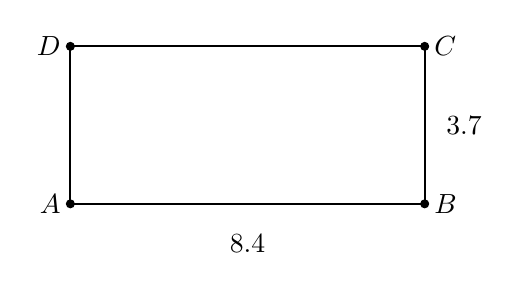
\begin{tikzpicture}
  \draw [-, thick] (0,0)--(4.5,0)--(4.5,2)--(0,2)--cycle;
  \draw [fill] (0,0) circle [radius=0.05] node[left]{$A$};
  \draw [fill] (4.5,0) circle [radius=0.05] node[right]{$B$};
  \draw [fill] (4.5,2) circle [radius=0.05] node[right]{$C$};
  \draw [fill] (0,2) circle [radius=0.05] node[left]{$D$};
  \node at (5, 1){3.7};
  \node at (2.25, -0.5){8.4};
\end{tikzpicture}
\end{flushleft} \vspace{1cm}  

\item The rectangle $BECA$ has an area of 143, with length $BE=13$. Find the width of the rectangle $EC$. (the drawing is not to scale)
\begin{flushleft}
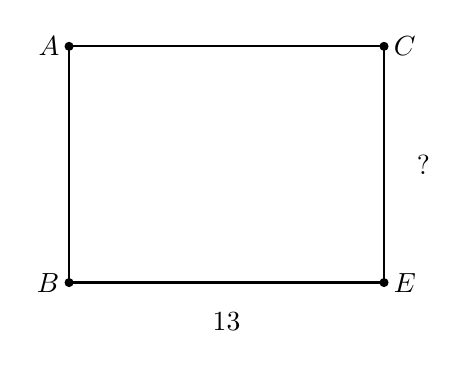
\begin{tikzpicture}
  \draw [-, thick] (0,0)--(4,0)--(4,3)--(0,3)--cycle;
  \draw [fill] (0,0) circle [radius=0.05] node[left]{$B$};
  \draw [fill] (4,0) circle [radius=0.05] node[right]{$E$};
  \draw [fill] (4,3) circle [radius=0.05] node[right]{$C$};
  \draw [fill] (0,3) circle [radius=0.05] node[left]{$A$};
  \node at (4.5, 1.5){?};
  \node at (2, -0.5){13};
\end{tikzpicture}
\end{flushleft} \vspace{2cm}  

\item Find the area of $\triangle CAT$. The altitude $h$ of the triangle is 4.9 centimeters and the base $CA=9.3$ cm.\\[0.5cm]
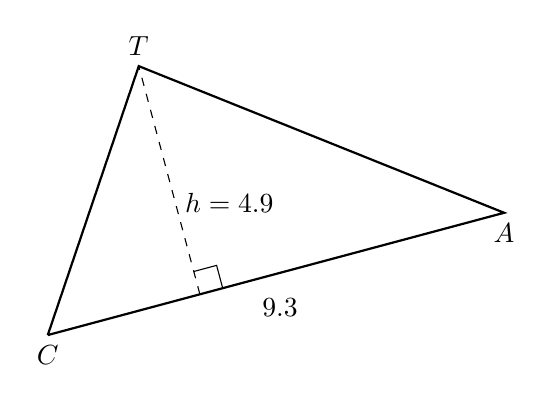
\begin{tikzpicture}[scale=1, rotate=15]
  \draw [thick]
    (2,0)node[below]{$C$}--
    (8,0)node[below]{$A$}--
    (4,3)node[above]{$T$} --(2,0);
 \draw [dashed] (4,0)--(4,3);
 \draw (4,0)++(0.3,0)--++(0,0.3)--+(-0.3,0);
 \node at (4,1.2)[right]{$h=4.9$};
 \node at (5,-0.2)[below]{$9.3$};
\end{tikzpicture} \vspace{1.0cm}

\newpage

\item One side of the $\triangle ABC$ has a length $AB=12$. The triangle's area is 30. Find the length of the altitude $h$ of the triangle to vertex $C$ and perpendicular to side $\overline{AB}$.\\[0.5cm]
  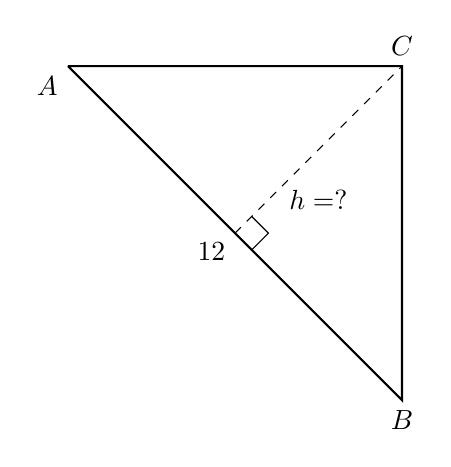
\begin{tikzpicture}[scale=1, rotate=-45]
    \draw [thick]
      (2,0)node[below left]{$A$}--
      (8,0)node[below]{$B$}--
      (5,3)node[above]{$C$} --(2,0);
  \draw [dashed] (5,0)--(5,3);
  \draw (5,0)++(0.3,0)--++(0,0.3)--+(-0.3,0);
  \node at (5.1,0.7)[right]{$h=?$};
  \node at (5,0)[below left]{$12$};
  \end{tikzpicture} \vspace{1.0cm}


\item Given $\overleftrightarrow{RS}$ as shown on the number line, with $R=-2.0$ and $S=4.2$. \\[20pt] % Midpoint
  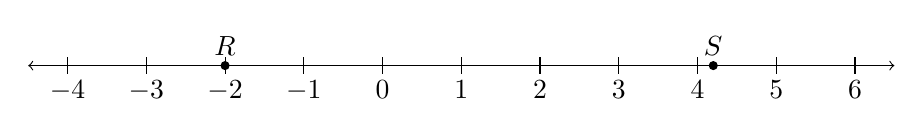
\begin{tikzpicture}
    \draw [<->] (-4.5,0)--(6.5,0);
    \foreach \x in {-4,...,6} %2 leading for diff!=1
      \draw[shift={(\x,0)},color=black] (0pt,-3pt) -- (0pt,3pt) node[below=5pt]  {$\x$};
      \draw [fill] (-2.0,0) circle [radius=0.05] node[above] {$R$};
      \draw [fill] (4.2,0) circle [radius=0.05] node[above] {$S$};
  \end{tikzpicture}
  \begin{enumerate}
    \item What is the exact distance on the number line between the points $R$ and $S$? \vspace{3cm} 
    \item The point $T$ bisects $\overline{RS}$. Find the value of $T$, and mark and label it on the numberline $\overleftrightarrow{RS}$ shown above. 
  \end{enumerate} \vspace{3cm}  
  
\newpage

\item Complete the construction of a perpendicular bisector of $\overline{AB}$. Label the midpoint $M$. Show all construction marks, but make no extra lines. \vspace{2cm}
  \begin{center}
  \begin{tikzpicture}
    \draw [-, thick] (0,0)--(4,5);
    \draw [fill] (0,0) circle [radius=0.05] node[below right]{$A$};
    \draw [fill] (4,5) circle [radius=0.05] node[above left]{$B$};
  \end{tikzpicture}
  \end{center} \vspace{4cm}

\item Accurately draw a square that is 5 centimeters on each side.

\newpage

\item Given $\overline{ABC}$, $AB=6 \frac{2}{5}$, and $AC=9$.\\ [0.5cm]
  Find ${BC}$.\\[1.5cm]
      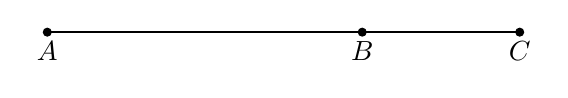
\begin{tikzpicture}
        \draw [-, thick] (1,0)--(7,0);
        \draw [fill] (1,0) circle [radius=0.05] node[below]{$A$};
        \draw [fill] (5,0) circle [radius=0.05] node[below]{$B$};
        \draw [fill] (7,0) circle [radius=0.05] node[below]{$C$};
      \end{tikzpicture}\\[1.5cm]
      The postulate used in this problem is the \rule{6cm}{0.15mm}.
      \vspace{1.5cm}

\item Given the diagram shown below. \vspace{0.25cm}
  \begin{enumerate}
    \item  Measure the angle $AEB$. $m \angle AEB = $ \rule{4cm}{0.15mm} \bigskip
    \item Name an angle that is complementary to $\angle DEB$: \rule{4cm}{0.15mm} \bigskip
    \item Name a pair of opposite rays: \rule{4cm}{0.15mm}
  \end{enumerate}
  \vspace{1cm}
  \begin{center}
  \begin{tikzpicture}[scale=1.3, rotate=-30]
    \draw [->, thick] (0,0)--(25:6);
    \draw [<->, thick] (-5,0)--(6,0);
    \draw [->, thick] (0,0)--(0,3);
    \draw (0,0)++(0.3,0)--++(0,0.3)--+(-0.3,0);
    %\draw [fill] (-1,2.5) circle [radius=0.05] node[left ]{$B$};
    \draw [fill] (25:4) circle [radius=0.05] node[below right]{$B$};
    \draw [fill] (-4,0) circle [radius=0.05] node[below]{$A$};
    \draw [fill] (0,0) circle [radius=0.05] node[below left]{$E$};
    \draw [fill] (0,2) circle [radius=0.05] node[left]{$C$};
    \draw [fill] (4,0) circle [radius=0.05] node[below]{$D$};
  \end{tikzpicture}
  \end{center}
  
\newpage 

\item Find the perimeter $P$ of the shape shown below, given the side lengths marked (not drawn to scale). All angles are $90^\circ$. Completely mark the diagram with the two missing lengths and show an equation for $P$ as a sum of each side's length.
  \begin{flushleft}
  \begin{tikzpicture}
    \draw [-, thick] (1,0)--(5,0)--(5,2)--(3,2)--(3,3)--(1,3)--cycle;
    %\draw [fill] (0,0) circle [radius=0.05] node[left]{$A$};
    %\draw [fill] (7,0) circle [radius=0.05] node[right]{$B$};
    %\draw [fill] (7,2) circle [radius=0.05] node[right]{$C$};
    %\draw [fill] (0,2) circle [radius=0.05] node[left]{$D$};
    \node at (5.5, 1){7};
    \node at (2.5, 3.5){8};
    \node at (3.5, -0.5){14};
    \node at (0.5, 1.5){10};
  \end{tikzpicture}
  \end{flushleft} \vspace{2cm}

\item Find the perimeter of a square with side length 7.25. \vspace{3cm}

\item Given two complementary angles, $m\angle A = 5x+14$ and $m\angle B = 3x-12$. Find the measure of $\angle B$. Check your solution. \vspace{3.5cm} 
 
\newpage
\item Complete the construction of an equilateral triangle with one side as $\overline{XY}$. Show all construction marks, but make no extra lines. \vspace{3cm}
  \begin{center}
  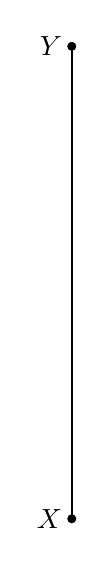
\begin{tikzpicture}
    \draw [-, thick] (0,0)--(0,6);
    \draw [fill] (0,0) circle [radius=0.05] node[left]{$X$};
    \draw [fill] (0,6) circle [radius=0.05] node[left]{$Y$};
  \end{tikzpicture}
  \end{center} \vspace{3cm}
  \begin{enumerate}
    \item Identify two circles in the construction. For each, name the center of the circle and the radius.  \vspace{3cm}
    \item Assuming that the third vertex of the triangle is point $Z$, explain why the distance from $X$ to $Z$ is the same as the distance from $X$ to $Y$.
  \end{enumerate}

\newpage
\subsubsection*{Complete all steps for full credit: the drawing to the top right, an equation and solution for $x$ on the left, followed by the answer to the question. Write the check to the bottom right.}

\item Given the collinear points $P$, $Q$, and $R$, with $PQ=3x+4$, $QR=2x+2$, and $PR=4x+10$. Find ${PR}$.
  \vspace{9cm}

\item Angles $M$ and $N$ are supplementary. $m\angle M = x+29$ and $m\angle N = 3x-9$. Find $m\angle N$. \vspace{7cm}


\newpage

\item Given that $E$ bisects $\overline{DF}$. $DE=12x-5$, $EF=9x+4$. Find ${EF}$.
  \vspace{9cm}

  \emph{Write the term that best completes each statement.}
\item Two or more line segments of equal measure are \rule{4cm}{0.15mm} \bigskip

\item Points that are located on the same line are \rule{4cm}{0.15mm} \\[15pt]

\item \emph{Factor and solve for $x$.}
  \begin{enumerate}
    \begin{multicols}{2}
        \item $x^2+8x+7=0$
        \item $x^2+7x=18$
    \end{multicols}
  \end{enumerate}
  
\newpage
\subsubsection*{Early finishers, spicy}

\item Complete the construction of a line perpendicular to line $l$ through the point $P$. Show all construction marks, but make no extra lines. \vspace{2cm}
  \begin{center}
  \begin{tikzpicture}
    \draw [<->, thick] (-5,0)--(7,0)node[below]{$l$}--(8,0);
    \draw [fill] (3,3) circle [radius=0.05] node[above left]{$P$};
  \end{tikzpicture}
  \end{center} \vspace{6cm}

\item The perimeter of a square is 52 cm. Find the area of the square.

\newpage
\item Given $\overleftrightarrow{FG}$ as shown on the number line, with $F=-2.5$ and $G=7.5$. \\[20pt] % Midpoint
  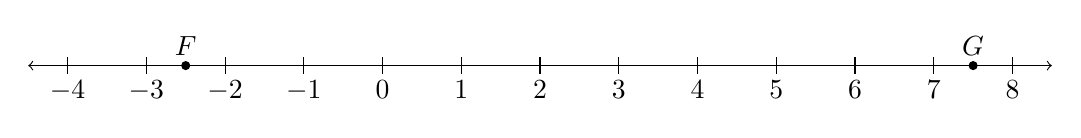
\begin{tikzpicture}
    \draw [<->] (-4.5,0)--(8.5,0);
    \foreach \x in {-4,...,8} %2 leading for diff!=1
      \draw[shift={(\x,0)},color=black] (0pt,-3pt) -- (0pt,3pt) node[below=5pt]  {$\x$};
      \draw [fill] (-2.5,0) circle [radius=0.05] node[above] {$F$};
      \draw [fill] (7.5,0) circle [radius=0.05] node[above] {$G$};
  \end{tikzpicture}\\[5pt]
  The point $H$ is $\frac{3}{4}$ of the way from $F$ to $G$. Find the value of $H$, and mark and label it on the numberline $\overleftrightarrow{FG}$. 
  \vspace{6cm}

\item The shape shown below is composed of straight lines and right angles, with some lengths as marked. Find the area of the figure. Show your work.
  \begin{flushleft}
  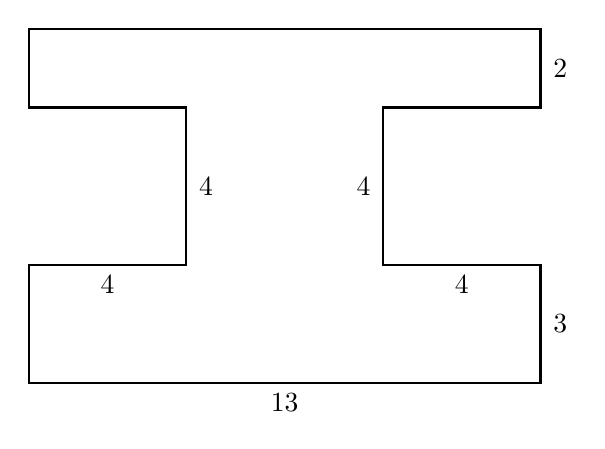
\begin{tikzpicture}[scale=0.5]
    \draw [-, thick] (0,0)--(13,0)--(13,3)--(9,3)--(9,7)--(13,7)--
    (13, 9)--(0,9)--(0,7)--(4,7)--(4,3)--(0,3)--cycle;
    %\draw [fill] (0,0) circle [radius=0.05] node[left]{$A$};
    %\draw [fill] (7,0) circle [radius=0.05] node[right]{$B$};
    %\draw [fill] (7,2) circle [radius=0.05] node[right]{$C$};
    %\draw [fill] (0,2) circle [radius=0.05] node[left]{$D$};
    \node at (4.5, 5){4};
    \node at (2, 2.5){4};
    \node at (8.5, 5){4};
    \node at (11, 2.5){4};
    \node at (6.5, -0.5){13};
    \node at (13.5, 1.5){3};
    \node at (13.5, 8){2};
  \end{tikzpicture}
  \end{flushleft} \vspace{2cm}

\newpage

\item The length of the given rectangle is 12 more than the width. Its area is 64. Find the length and width of the rectangle using an algebraic method.\\[5pt]
  (the drawing is not to scale)
  \begin{flushleft}
  \begin{tikzpicture}
    \draw [-, thick] (0,0)--(4.5,0)--(4.5,2)--(0,2)--cycle;
    \node at (5, 1){x};
    \node at (2.25, -0.5){$x+12$};
  \end{tikzpicture}
  \end{flushleft} \vspace{5cm}

\item The circle with center $B$ is shown below with diameter $\overline{AC}$ and radius $\overline{BD}$. Given $BC=7x-3$ and $BD=5x+9$. Find the diameter of the circle.
  \begin{flushleft}
  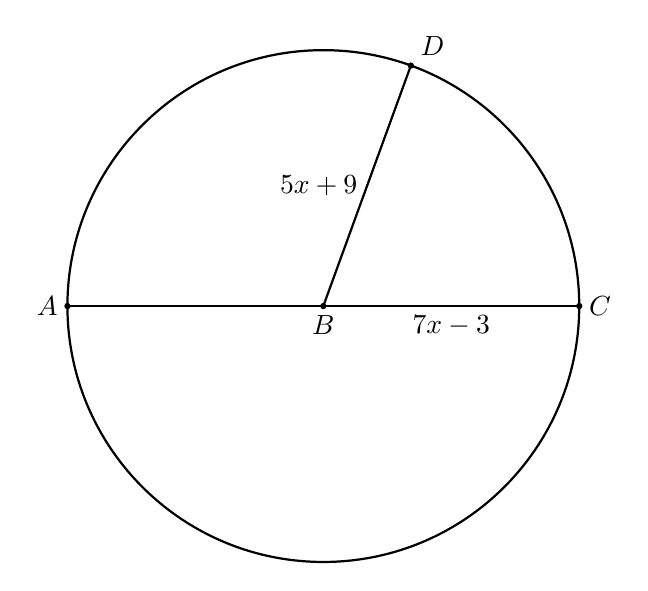
\begin{tikzpicture}[scale=0.65]
    \draw [thick] (0,0) circle [radius=5];
    \draw [-, thick] (-5,0)--(0,0)--(5,0);
    \draw [-, thick] (0,0)--(70:5);
    \draw [fill] (-5,0) circle [radius=0.05] node[left]{$A$};
    \draw [fill] (0,0) circle [radius=0.05] node[below]{$B$};
    \draw [fill] (5,0) circle [radius=0.05] node[right]{$C$};
    \draw [fill] (70:5) circle [radius=0.05] node[above right]{$D$};
    \node at (70:2.5)[left]{$5x+9$};
    \node at (2.5, 0)[below]{$7x-3$};
  \end{tikzpicture}
  \end{flushleft} \vspace{2cm}

\end{enumerate}
\end{document}